\chapter{Environmental noise}

Environmental noise refers to any signal originating from outside the structure of a \ac{GW} detector that can impact the detector's sensitivity or disrupt its ability to achieve and maintain lock~\cite{Effler2015,Nguyen2021}.
The effects of environmental noise on detector sensitivity can range from persistent excess noise in the \ac{GW} strain data, to short-duration transient signals, or \textit{glitches}.

One goal of studying environmental noise is to aid in the validation of \ac{GW} events.
Due to the sophisticated nature of the search pipelines used to detect gravitational waves in the \ac{LIGO} data, environmental glitches are highly unlikely to fully account for a \ac{GW} event candidate.
That said, glitches capable of influencing analyses occur frequently at both observatories.

Unlike instrumental noise, environmental noise can potentially be correlated between different detectors, i.e. stemming from a common source as opposed to stemming from chance coincidence.
Such correlated noise is not accounted for in the estimation of false-alarm probabilities, which is done by time-shifting background data from each \ac{LIGO} detector to produce long stretches of coincident background.

Environmental noise is particularly important in searches for un-modeled sources of gravitational waves, as these look for excess power without the use of waveform templates.
Even for highly significant \ac{CBC} events, contamination of the strain data can be detrimental to parameter estimation analyses that infer source properties from the morphology of the event.
Thus it is important to have a quantitative solution for identifying and evaluating the impact of environmental transients when they occur coincide with candidate events.

The second goal is to improve the sensitivity and performance of the detector by localizing noise sources and coupling mechanisms. Once tracked down, they can be mitigated by eliminating the noise sources, attenuating the propagation of the signal, or modifying the detector itself.

\section{Sources of environmental noise}

The environment can influence a \ac{GW} detector through physical contact (via vibrations or temperature fluctuations), electromagnetic waves, static electric and magnetic fields, and possibly high-energy radiation.

Vibrations can affect the data by directly moving the test masses.
They can also cause modulate the paths of light that is scattered off of surfaces inside the interferometer, or introduce fluctuations in the alignment of the input laser beam.

\section{The PEM sensor array}

\begin{figure}[h!]
	\centering
	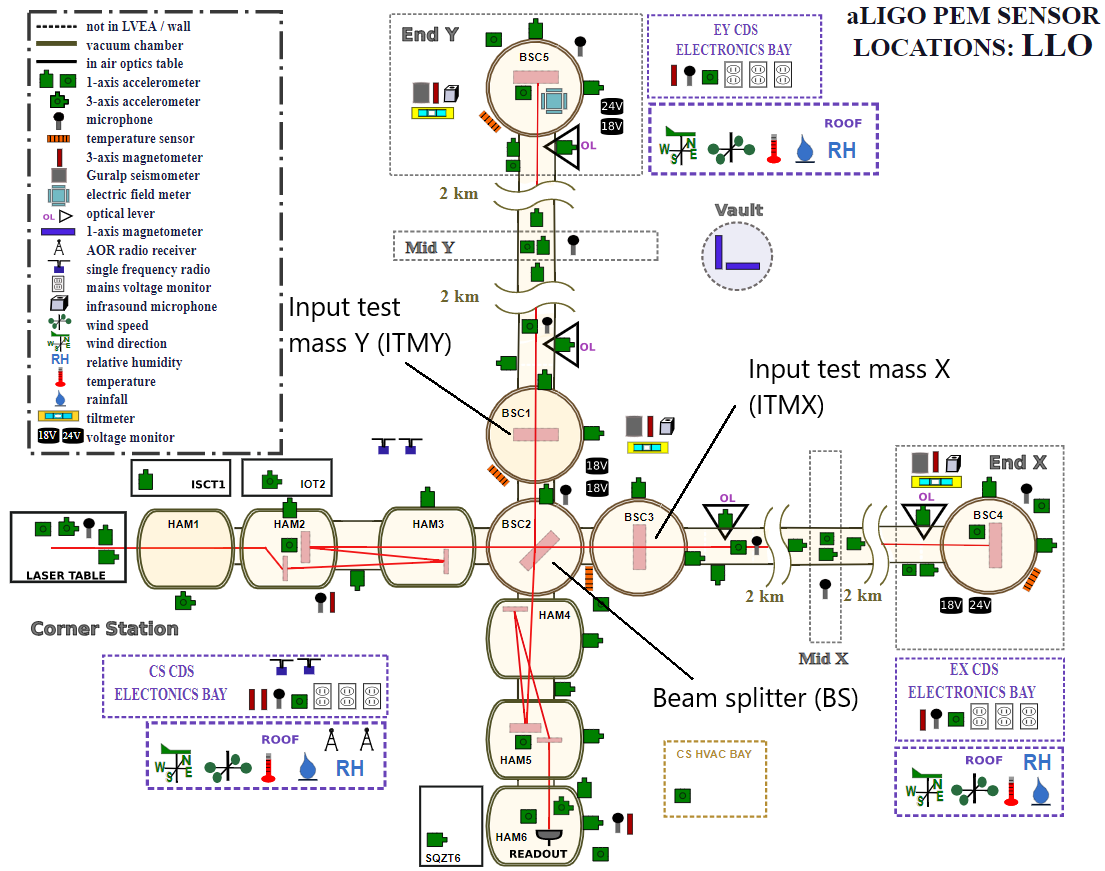
\includegraphics[width=\textwidth]{figures/channels.png}
	\caption{
		The PEM system layout at LLO during O3, as seen on the PEM public website.}
	\label{fig:channels}
\end{figure}

Understanding environmental influences on the detectors requires comprehensive monitoring of its physical surroundings.
This is done through the \ac{PEM} system of auxiliary sensors (Figure~\ref{fig:channels}), which consists of accelerometers for high-frequency vibrations (between tens to thousands of Hertz), seismometers for low-frequency vibrations (up to tens of Hertz), microphones, magnetometers, voltage monitors that measure the voltage of electric power supplied to the detector sites, radio-frequency (RF) receivers, a cosmic-ray detector for high-energy particles, and wind, temperature and humidity sensors.
Detailed information on \ac{PEM} sensors, including example background spectra and calibration data, can be found on the \ac{PEM} website, PEM.LIGO.org~\cite{PEM_website}.

\section{Tests of environmental coupling}\label{subsec:injections}

\begin{figure}[h!]
	\centering
	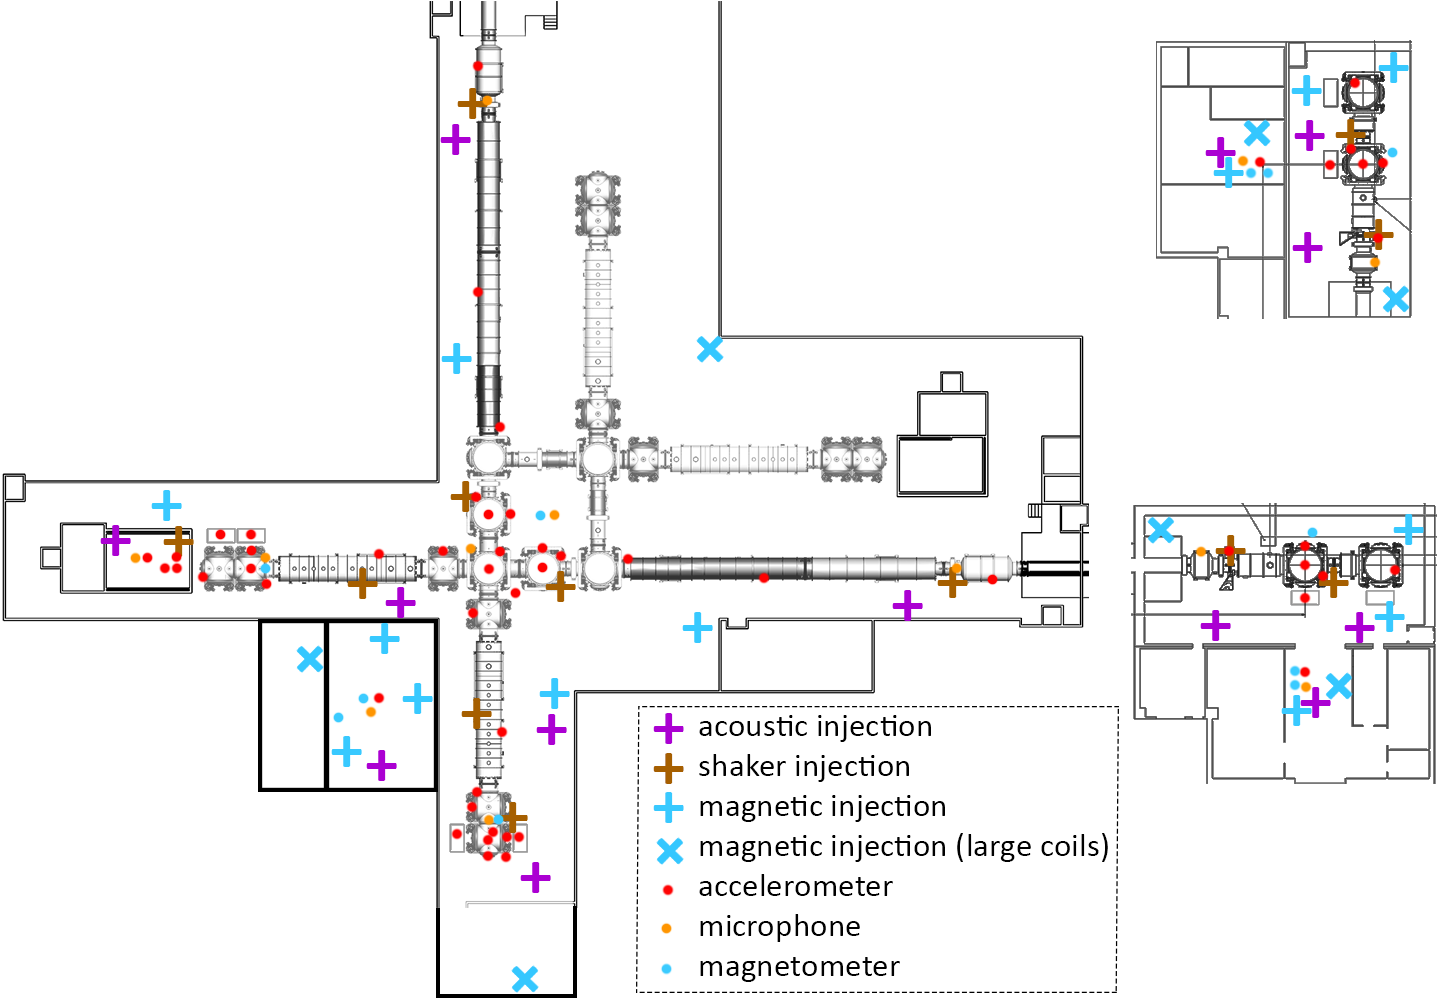
\includegraphics[width=\textwidth]{figures/injection-map.png}
	\caption{
		Standard locations for vibration and magnetic injections at the LHO corner station (left), Y end station (top right), and X end stations (bottom right).}
	\label{fig:injection_map}
\end{figure}

The effect of environmental influences on the sensitivity of a \ac{GW} detector can be studied by making noise \textit{injections}.
These are signals produced by human-operated sources with the intention of replicating environmental disturbances with sufficient amplitude to produce excess noise in the \ac{DARM} spectrum.
The amplitude of the excess, combined with measurements of the input signal, can be used to quantify the coupling behavior (Section~\ref{sec:cf}).
The most common examples are acoustic injections, generated using speakers, seismic injections generated by vibrational shakers, and magnetic field injections generated by electrical current loops.

At each observatory we inject from 13 locations with acoustic injections, about 12 with shaking injections, and 15 with small-coil magnetic injections, with 7 large-coil magnetic injection locations planned for \ac{O4} (as explained in Section~\ref{sec:magnetic-injections}).
The number and locations of shaker injections vary between injection campaigns. For all injection types, multiple injections are made at each location in order to focus on different frequency bands.
Additionally, impulse injections (not shown) are made at locations where vibrational injections have revealed strong coupling sites.

\begin{table}[h!]
\caption{\label{tab:injectors}Specifications for injection equipment.}
\begin{tabular}{|ll|}
	\hline
	Equipment & Injection type \\
	\hline
	Custom enclosure with two 14-in. speakers & Acoustic\\
	Various smaller speakers & Acoustic\\
	APS 113 Electro-Seis\reg Long Stroke Shaker~\cite{big_shaker} & Vibrational\\
	Piezosystem\reg~\cite{piezo} shaker with custom reaction mass & Vibrational\\
	Br\"uel \& Kj\ae r\reg~\cite{bk} EM shaker with custom reaction mass & Vibrational\\
	1\,m diameter copper coil (100\,turns) & Magnetic\\
	3\,x\,3\,m and 5\,x\,5\,m coils (80-100\,turns) & Magnetic\\ \hline
\end{tabular}
\end{table}


Injection locations are chosen to best mimic disturbances from outside the detector (Figure~\ref{fig:injection_map}).
To do so we choose them to be as far from the detector and environmental sensors as possible, but we are usually limited by the size of the detector sites themselves (some injections can be made from outside).
Time dedicated to these tests has to be balanced against other instrumental work and observing time, which leads to a trade-off between measurement uncertainty and coverage.
We perform injections from as many locations as time allows in order to maximize coverage of potential coupling sites.
Increased time allocation toward environmental studies in recent years has allowed for a significant increase in the number of injection locations.
Table~\ref{tab:injectors} summarizes the current equipment used and Figure~\ref{fig:injection_equipment} shows photos of some of the equipment.

\begin{figure}[h!]
	\centering
	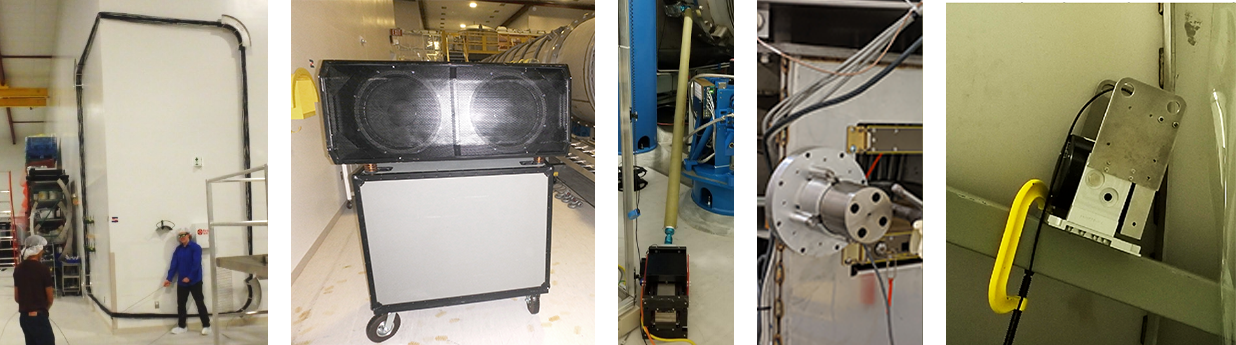
\includegraphics[width=\textwidth]{figures/injection-equipment.png}
	\caption{Injection equipment photos. From left to right: wall-mounted magnetic field injection coil; 14-in. speakers; APS 113 shaker connected to the door of a vacuum chamber by a rigid fiberglass rod; modified Piezosystem shaker clamped to an electronics rack; modified B\&K shaker clamped to a beam tube support.}
	\label{fig:injection_equipment}
\end{figure}

\subsection{Vibrational injections}

Acoustic injections are produced by large speakers. For the corner stations, a pair of speakers mounted on a vibrationally isolated cart (to minimize ground-based vibrational signals) are used.
Typically, the injection signal is white noise band-passed between 20-2000\,Hz, with narrower bands being used for special follow-up of particular coupling sites.

Seismic injections at low frequency (up to tens of Hertz) during \ac{iLIGO} were performed with small electromagnetic and piezoelectric shakers~\cite{bk, piezo} and a weighted cart.
A large shaker~\cite{big_shaker} has been used since the beginning of noise studies for \ac{O3}.
The large shaker can impart up to 133\,N of sine force and a peak-to-peak displacement of 158\,mm, compared to the electromagnetic shaker which imparts up to 45\,N of force and a displacement of 8\,mm.
While smaller shakers can be directly clamped to the interferometer supports, a rigid fiberglass rod is used to connect the large shaker to the interferometer.
This has an added benefit of being better able to adjust the direction of the actuation by angling the rod and shaker accordingly.

Two new injection techniques have been developed for localizing vibration coupling sites connected to the vacuum enclosure, such as locations on the vacuum enclosure that reflect scattered light.
The techniques rely on the slow propagation speeds (hundreds of meters per second) of vibrations on the steel vacuum enclosure walls or, for acoustic injections, in air.
These two techniques aided in the localization of a coupling site that was producing a 48\,Hz peak in the \ac{GW} channel throughout the first half of O3, as discussed in Section~\ref{sec:scattering}.

\subsubsection{Beating-shakers technique}

The beating-shakers technique is narrow-band, and involves vibrating the vacuum enclosure at two slightly different frequencies, each injected from a shaker or a speaker at a different location (e.g. a shaker at one location injects a sine wave at frequency $f$ and a shaker at the other location injections at frequency $f + 0.01$\,Hz).
The two injections are adjusted in amplitude to produce strong beats in the \ac{GW} channel.

Because the injection locations are different, the relative phase of the two injected signals varies with location on the vacuum enclosure.
As a result, the phase of the beat envelope varies with position, and different sites experience maximum chamber wall motion at different times.
The sites with accelerometer signals that have the same beat envelope phase as the \ac{DARM} signal are candidates for the scattering sites on the vacuum enclosure walls.
Other sensors that are not near the coupling site may also match the phase by chance, but these false positives can be rejected by varying the locations of the shakers.

Figure~\ref{fig:beats} provides an example of a beating-shakers injection used to localize the coupling site responsible for a 48\hyp Hz noise peak in the \ac{DARM} spectrum.
The shakers were injecting at 48 and 48.01\,Hz. The Y-axes of the spectrograms are centered along at 48\,Hz and show the combined signal in each sensor modulating at the beat frequency (0.01\,Hz).
This set of spectrograms suggests that the accelerometers on the \ac{ITM} chambers and the Y-axis HAM2 accelerometer are likely not close to the true coupling location, since the beat envelopes are the furthest offset from the beat envelope in the \ac{DARM} response.
Multiple other injections were made (not shown here) with varying shaker locations in order to rule out other sensors until the most likely candidate remaining was the HAM3 Y-axis accelerometer.
Black glass was used to block scattered light at this location and the peak was eliminated for the second half of the O3 observation run.

\begin{figure}[h!]
	\centering
	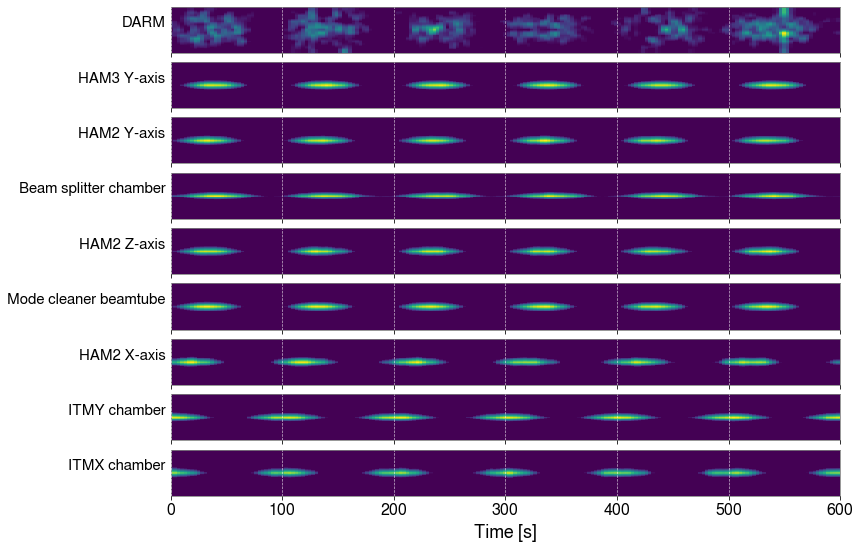
\includegraphics[width=\textwidth]{figures/beat-spectrograms.png}
	\caption{
		Spectrograms of DARM and various accelerometers near the input arm and beam splitter showing a beating-shakers injection at 48\,Hz.}
	\label{fig:beats}
\end{figure}

\subsubsection{Impulse injections}

The second injection technique, which is broad band, involves propagation delays in impulse injections.
Impulse injections are performed by striking the vacuum enclosure directly with enough force to produce a transient in the \ac{GW} channel and in nearby accelerometers.
The vibrational impulse propagates through the structure of the vacuum enclosure, arriving at different accelerometers and coupling sites at different times.

We can distinguish these arrival times because the propagation velocity is much slower than in solid material, and is only roughly 300\,m/s in our case. Using time series plots, the arrival time of the impulse in the \ac{GW} channel is compared to the arrival time of the impulse in multiple accelerometers (Figure~\ref{fig:impulse}, left).
The accelerometers that show the same arrival time as in the \ac{GW} channel are more likely to be near a coupling site than those that observe the impulse much earlier or later.
Again, varying the location of the injection eliminates sensors that match the detector time-of-arrival by chance but are actually far from the coupling site.

An additional consistency check is that the coupling of accelerometers near the coupling site will vary less between different impulse locations than that of accelerometers far from the coupling site.
Finally, if the accelerometer is at the coupling site, the impulse in the \ac{GW} channel will have a resonance structure that is similar to the resonance structure of the accelerometer signal, which can be judged from spectrograms (Figure~\ref{fig:impulse}, right).

Example time series and spectrograms are provided in Figure~\ref{fig:impulse}.
The plots show a single impulse injection signal in the \ac{GW} channel and in various output optics accelerometers.
Multiple sensors observe an impulse time-of-arrival matching that of the \ac{GW} channel, but repeating the injection from various other locations rules out sensors that do not match it consistently across multiple injections.
In this case the septum (separating the HAM5 and HAM6 chambers) accelerometer signal matches the \ac{DARM} signal most consistently (other injections not shown for brevity).

Spectrograms of the same impulse injection for \ac{DARM} and the three sensors with the closest matching time-of-arrival to that of \ac{DARM} reveals similarities between the frequency structure of the septum accelerometer signal and that of \ac{DARM}.
This provides further support that the septum is the dominant coupling site in the output arm.

\begin{figure}[h!]
	\centering
	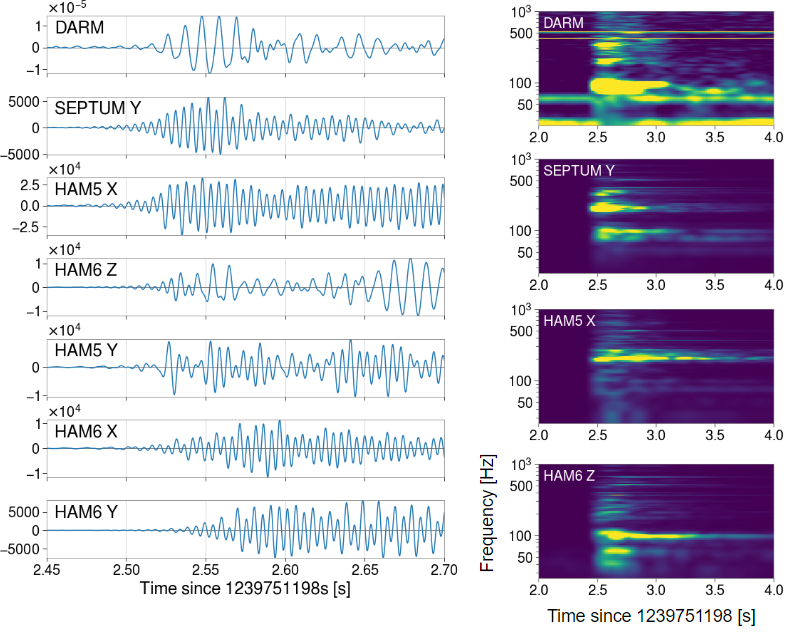
\includegraphics[width=\textwidth]{figures/impulse.png}
	\caption{
		Time series (left) and spectrograms (right) of a vibrational impulse injection produced at the output arm of the LHO detector.}
	\label{fig:impulse}
\end{figure}


\subsection{Magnetic injections}\label{sec:magnetic-injections}

Improvements have also been made to the magnetic field injection equipment. In order to generate fields strong enough to couple into the \ac{GW} channel using the 1\,m magnetic field coils built during \ac{iLIGO}~\cite{Effler2015}, we must focus the power of the coil into narrow bands and combs instead of injecting broadband signals. This was sufficient in \ac{iLIGO} when strong magnetic coupling occurred primarily through permanent magnets. However, due to the removal of permanent magnets from the test masses, coupling from those sources has decreased and cables and connectors have become the dominant coupling sites above about 80\,Hz, introducing more structure to the coupling functions and requiring stronger injections.

\begin{figure}[h!]
	\centering
	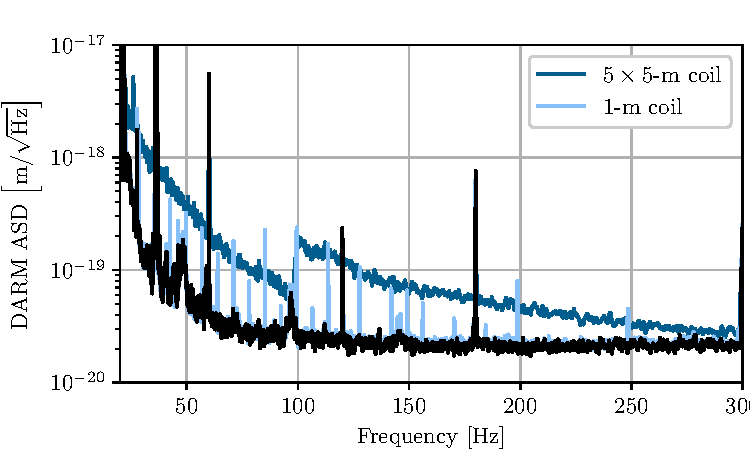
\includegraphics{figures/wallcoil.pdf}
	\caption{
		Comparison of the old small-coil comb magnetic field injections with the new large-coil broadband injections.}
	\label{fig:wallcoil}
\end{figure}

To achieve high-amplitude broadband magnetic injections, seven wall-mounted coils, each one a 3\,m x 3\,m or 5\,m x 5\,m square of 80-100\,turns, are being installed at each site; three at the corner station and two at each end station. These coils are fixed in place and can be operated remotely, allowing for weekly injections to monitor variations in magnetic coupling caused by changes to electronics. Figure~\ref{fig:wallcoil} compares the old and new magnetic injections. Some coils were installed and operated at the sites during O3; the project will be completed by the start of O4.

\section{Coupling functions}\label{sec:cf}

\subsection{Single coupling site, sensor, and injection}

Suppose there exists exactly one coupling site, i.e. one location at which incident environmental signals result in excess noise in the \ac{GW} strain data.
Suppose also that a sensor is placed at the location of the coupling site, and a noise injection is performed that produces a signal observable by the sensor and the interferometer readout.
The coupling mechanism can be modeled in the frequency domain as a linear system:

\begin{equation}\label{eq:cf_model}
	h(f) = C(f) x(f),
\end{equation}
where $h(f)$ is the amplitude of the detector response, $x$ is the amplitude of the injection signal as measured by the sensor, and $C(f)$ is the \textit{coupling function}, which represents the amplitude of gravitational wave strain noise per unit amplitude in the sensor.
By convention, the strain is typically converted to \ac{DARM}, in meters, in which case $C(f)$ represents  test mass displacement per calibrated unit of sensor amplitude.
If the injection signal is an acoustic signal and the sensor a microphone measuring in Pa, for instance, the acoustic coupling function is in units of m/Pa.

The coupling function can be computed by measuring the \acp{ASD} of the \ac{GW} detector and the witness sensor during the time of the injection (\textit{injection time}) to their \acp{ASD} during a time when both are at observation-mode noise levels (\textit{background time}).
The coupling function at some frequency $f$ is given by the ratio of excess power in the detector to the ratio of excess power in the sensor~\cite{Kruk_2016, pem_code}:

\begin{equation}\label{eq:cf}
	\mathrm{C}(f) = \sqrt{\frac{[h_{\textrm{inj}}(f)]^2 - [h_{\textrm{bkg}}(f)]^2}{[x_{\textrm{inj}}(f)]^2 - [x_{\textrm{bkg}}(f)]^2}}.
\end{equation}
Here $x_{\textrm{bkg}}(f)$ and $x_{\textrm{inj}}(f)$ are the \acp{ASD} of the witness sensor at background and injection times, respectively, and $h_{\textrm{bkg}}(f)$ and $h_{\textrm{inj}}(f)$ are the \ac{GW} detector \acp{ASD} at background and injection times.
The coupling function for a sensor is produced by computing a \textit{coupling factor} at each frequency bin in which excess noise is detectable in the sensor.

\subsection{Multiple coupling sites, sensors, and injections}

Suppose now there are multiple coupling sites, and a sensor is placed at the location of each site.
The detector response to an environmental signal now becomes a linear combination of the sensor signals and their sensor-specific coupling functions:

\begin{equation}\label{eq:cf_model_expanded}
	h(f) = \sum_{j=1}^{m} \mathrm{C}_j(f) x_{j}(f),
\end{equation}
Solving for the coupling function now would require multiple injections instead of just one, resulting in a system of $n$ equations with $m$ unknown coupling functions, where $n$ and $m$ are the numbers of injections and sensors, respectively:

\begin{equation}\label{eq:cf_full}
	h_i(f) = \sum_{j=1}^{m} \mathrm{C}_j(f) x_{ij}(f).
\end{equation}
Here $h_i(f)$ is the detector response during injection $i$, $x_{ij}(f)$ is the amplitude measured by sensor $j$ during injection $i$, and $\mathrm{C}_j(f)$ is the coupling function of sensor $j$.
In principle, Equation~\ref{eq:cf_full} can be solved to determine the coupling functions of all sensors.

Thus far it has been assumed that the witness sensors are placed precisely at the locations of the coupling mechanisms, but such perfect placement is not realistically feasible given that there are an unknown number of coupling sites at unknown locations.
A sensor, even if it is near a coupling site, only measures the injection amplitude at its own location, not at the coupling location.
Therefore, when using real-world sensors, eq.~\ref{eq:cf} is only an estimate of the true coupling, and eq.~\ref{eq:cf_full} is not an exact model of all the coupling mechanisms.
Nevertheless, as explained above, sensors are distributed in order to maximize coverage of coupling sites and this has been sufficient for producing reliable coupling functions for all sensors, as discussed further in Section~\ref{subsec:uncertainties}.

\subsection{Solving the coupling equations}

One hurdle remains in attempting to solve~\ref{eq:cf_full}.
In practice, typically $n<m$ due to logistical constraints on the number of injections one could perform during a realistic time window, which makes the system of equations underdetermined.
Below are two approximation methods for determining $C_j(f)$ for all sensors.

\textit{Nearest-sensors approximation}.
One method of forcing $n=m$ is reducing the number of sensors in each each equation, by asserting $x_{ij}(f)=0$ for sensors that are sufficiently far from the source of injection $i$.
This can be done by ordering the sensors by distance from the injection source and applying the assertion to the $m-n$ farthest sensors.
Issues can arise if there are sensors that are never near enough to any injection source, causing them to zeroed out for all injections; this requires that injections be distributed such that each sensor is near enough to at least one injection.

\textit{Nearest-injection approximation}.
Instead of solving Equation~\ref{eq:cf_full} in full, one can approximate $\mathrm{C}_j(f)$ for each sensor independently of other sensors.
Given a sensor $j$, Equation~\ref{eq:cf} can be repurposed by replacing $x$ with $x_{ij}$ and $h$ with $h_i$ to compute a single-injection ``coupling function'' $\mathcal{C}_{ij}(f)$ for each injection:

\begin{equation}\label{eq:sicf}
	\mathcal{C}_{ij}(f) = \sqrt{\frac{[h_{i,\textrm{inj}}(f)]^2 - [h_{i,\textrm{bkg}}(f)]^2}{[x_{ij,\textrm{inj}}(f)]^2 - [x_{ij,\textrm{bkg}}(f)]^2}}.
\end{equation}
The closer an injection is to a sensor $i$, the more accurately $\mathcal{C}_{ij}(f)$ approximates $\mathrm{C}_j(f)$, since the detector response would be dominated by coupling near sensor $j$.
Therefore one can construct the sensor coupling function by choosing at each frequency bin the coupling factor corresponding to the nearest injection, determined by the highest sensor amplitude (using the assumption that injection amplitudes are equivalent).
That is, for a frequency $f_k$ and a set of injections $\mathcal{I}$, one can measure the sensor amplitudes $\{x_{ij}(f_k)\ |\ i \in \mathcal{I}\}$, compute the single-injection coupling functions $\{\mathcal{C}_{ij}(f_k)\ |\ i \in \mathcal{I}\}$, and construct the approximate sensor coupling function

\begin{equation}\label{eq:ccf}
	\widetilde{\mathrm{C}}_j(f_k) := \mathcal{C}_{lj}(f_k)\ \mathrm{where}\ l = \mathop{argmax}_{i\in\mathcal{I}}\ (x_{ij}(f_k)).
\end{equation}
If the distribution of injection locations provides sufficient coverage of sensor locations, then $\widetilde{\mathrm{C}}_j(f) \approx \mathrm{C}_j(f)$.
Shortcomings of this assumption are discussed in Section~\ref{subsec:uncertainties}.

Figure~\ref{fig:injection} provides an example of a coupling function measurement for a \ac{PSL} acoustic injection.
Figure~\ref{fig:composite} shows an estimated ambient noise based on an accelerometer coupling function constructed from five single-injection coupling functions.
For simplicity only five injections were used to produce this example, however in practice the number of injections performed near a sensor can be much higher.

\begin{figure}
	\centering
	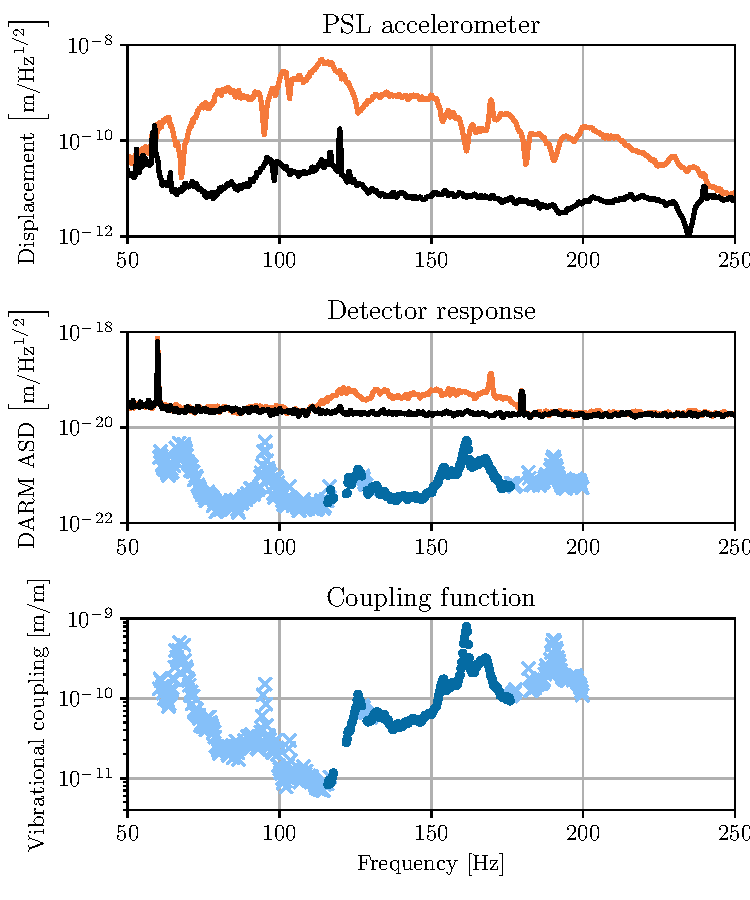
\includegraphics[width=\textwidth]{figures/injection-example.pdf}
	\caption{
		Example of a broadband acoustic noise injection and measurement of a single-injection coupling function.
		Top: displacement of an accelerometer in the PSL room during background time (black) and injection time (orange).
		Middle: DARM during background time (black) and injection time (orange).
		Estimated ambient levels for the accelerometer are shown as dark blue dots, with upper limits shown as light blue crosses.
		Bottom: single-injection coupling function used to produce estimated ambient above.}
	\label{fig:injection}
\end{figure}

Due to hardware limitations it can be possible for an injection signal to be strong enough to produce excess noise in a sensor \ac{ASD} but not in the \ac{GW} detector \ac{ASD}.
For frequency bins where this is the case, an upper limit on $\mathcal{C}_{ij}(f_k)$ can be established by assuming, as a worst-case scenario, that all of the detector noise at that frequency is produced by the coupling alone

\begin{equation}\label{eq:siul}
	\mathrm{C}_{ul}(f) = \frac{h_{i,\textrm{bkg}}(f)}{\sqrt{[x_{ij,\textrm{inj}}(f)]^2 - [x_{ij,\textrm{bkg}}(f)]^2}}.
\end{equation}
The larger the injection amplitude, the better this upper limit can be constrained.
The boundaries between measurements, upper limits, and null results are established by two \ac{ASD} ratio thresholds: a sensor threshold and a detector threshold.
Let $r_x := x_{ij,\textrm{inj}}(f) / x_{ij,\textrm{bkg}}(f)$ and $r_h := h_{i,\textrm{inj}}(f) / h_{i,\textrm{bkg}}(f)$ represent the injection signal-to-noise ratios if the sensor and \ac{GW} detector \acp{ASD}, respectively.
If $r_x \geq t_x$ and $r_h \geq t_h$, where $t_x$ is the sensor threshold and $t_h$ is the detector threshold, then a measurement is computed via eq.~\ref{eq:sicf}.
Otherwise, if $r_x \geq t_x$ but $r_h < t_h$, then eq.~\ref{eq:siul} is used to place an upper limit on the coupling.
If $r_x < t_x$ and $r_h < t_h$, then neither a measurement nor upper limit is computed.
The values of $t_x$ and $t_h$ are determined based on typical level of random fluctuations observed in the spectra, but often values of $t_x = 10$ and $t_h = 2$ are used for most types of sensors and injections.
The higher choice of $t_x$ is due to the environmental sensors being much more sensitive to random fluctuations in the ambient noise level than the interferometer is.

The coupling function as approximated in eq.~\ref{eq:ccf} is used for comparing coupling between different sensor locations and producing estimates of interferometer noise levels, e.g. as part of event validation (see Section~\ref{subsec:vetting}).
References to a sensor's coupling function will hereafter refer to this approximate quantity.
Figure~\ref{fig:composite} provides an example of an estimated ambient for an accelerometer on the HAM6 vacuum chamber (which houses the interferometer output optics).
The \ac{PEM} website provides coupling functions for all accelerometers, microphones, and magnetometers produced from the most recent campaign of injections~\cite{PEM_website}.

\begin{figure}[h!]
	\centering
	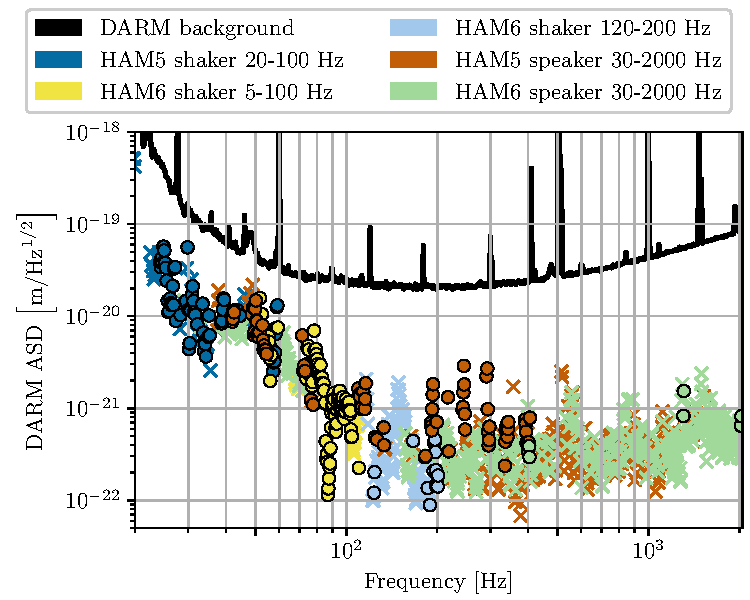
\includegraphics{figures/composite.pdf}
	\caption{
		Ambient noise level for the LHO HAM6 Y-axis accelerometer estimated from a composite coupling function, using acoustic and seismic injections near the output arm.}
	\label{fig:composite}
\end{figure}

\section{Uncertainties and limitations of coupling functions}\label{subsec:uncertainties}

\subsection{Comparison to transfer functions}

Environmental coupling is characterized using coupling functions instead of transfer functions because perfect coherence is not assumed in the system.
Low coherence can arise either due to non-linearity in the coupling or due to the spacing between the sensor and coupling site.
On a superficial level, a coupling function lacks a phase response component, representing only the magnitude response in the system.
Coupling functions also differ fundamentally from transfer functions in the sense that they do not assume the input signal to be the true actuation signal, but rather merely a witness of the actuation, while the actuation is in fact occurring at the location of the true coupling site.

\subsection{Assumptions about coupling mechanisms}

Equation~\ref{eq:cf} relies on two assumptions about the coupling mechanism.
First, the coupling is assumed to be linear in amplitude, e.g. doubling the amplitude of the injection would double the amplitude of the \ac{GW} detector response.
This is confirmed when performing injections by repeating them with different amplitudes and ensuring that the detector response scales proportionally with the injection amplitude.
Second, the coupling function ignores any up- or down-conversion of the signal between the sensor and the \ac{GW} detector.
Such non-linear coupling can be very significant for scattering noise and bilinear coupling, but is not accounted for in the estimates of linear coupling.
One way to check for non-linear coupling is by sweeping single frequency injections over time and searching for off-frequency responses in the \ac{GW} detector.
Frequency changes from non-linear coupling can be an issue in broadband injections where up- or down-converted noise in the interferometer readout appears in the injection band, resulting in artificially higher estimates at those frequencies.
We split broadband injections into smaller frequency bands to avoid this effect when necessary.
One approach for quantifying non-linear coupling is presented in Washimi et al.\ (2020)~\cite{Washimi_2020}.

\subsection{Hardware limitations}

\textit{Amplitude limitations}. To measure coupling, we inject signals large enough to produce a response in the detector, but the maximum amplitude of injections is limited by the sensitive range of the environmental sensors (saturation produces an overestimate of coupling).
This effectively limits how far below the detector noise background we can probe for coupling or establish upper limits.

\textit{Uncertainty due to injection locations}.
As mentioned above, the model in Equation~\ref{eq:cf_full} relies on the assumption that the environment is monitored at the coupling site.
The density of sensors is not great enough for this to be strictly true, especially if the source of the environmental signal is closer to the coupling site than the sensor is.
The detector response to an injection depends on the distance between the injection and coupling site, whereas the sensor response depends on the distance between the injection and sensor.
Varying the injection location therefore varies the relative scaling of the numerator and denominator of Equation~\ref{eq:sicf}, affecting the measurement of $\mathcal{C}_{ij}(f)$ and subsequently the sensor coupling function via Equation~\ref{eq:ccf}.
Therefore, a finite spacing of sensors leads to some degree of uncertainty in the coupling functions.
This uncertainty also propagates to projected noise levels in the \ac{GW} channel using these coupling functions.

\begin{figure}[h!]
	\centering
	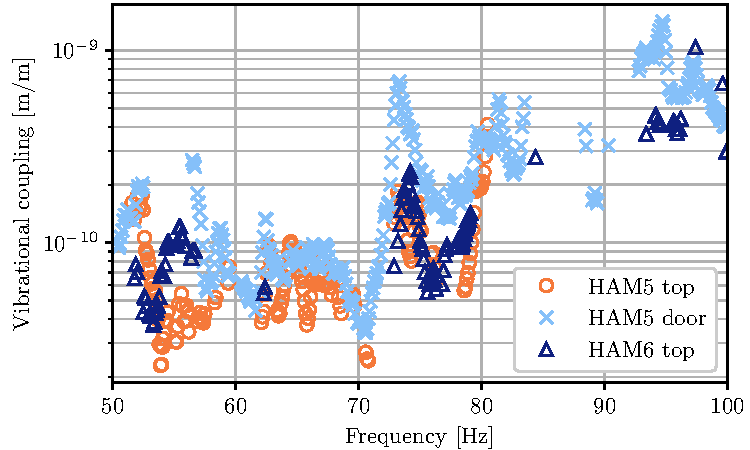
\includegraphics[width=\textwidth]{figures/injection-locations.pdf}
	\caption{
		Single-injection coupling functions (upper limits not shown) for the HAM5 Y-axis accelerometer for three different shaker injection locations (on top of HAM5, on top of HAM6, and on the HAM5 chamber door).}
	\label{fig:injection_locations}
\end{figure}

Since the uncertainty manifests as a multiplicative scaling of $\mathcal{C}_{ij}(f)$, it can be described by computing a geometric standard deviation of $\mathcal{C}_{ij}(f)$ for a single sensor over a range of injection locations, at each frequency bin.
Figure~\ref{fig:injection_locations} shows single-injection coupling functions for an accelerometer measured from shaker injections produced from three locations (the distribution of injection locations is discussed in Section~\ref{subsec:injections}.
Since the injection locations are close enough to the accelerometer, it can be assumed that the variance is primarily due to finite spacing effect.
Averaged across all frequency bins, the geometric standard deviation between injection locations is 1.4, i.e. coupling functions measured from vibrational injections can be expected to vary by a factor of 1.4 when measured by different injection locations.

\begin{figure}[h!]
	\centering
%	\includegraphics[width=\textwidth]{figures/injection-locations-mag.pdf}
	\caption{
		Single-injection coupling functions (upper limits not shown) for various magnetometers and various injections at both observatories.}
	\label{fig:injection_locations_mag}
\end{figure}

A similar study was performed combining geometric standard deviations for various magnetometers at both observatories.
There are fewer magnetic injection locations to use for the comparison, but since coupling can be measured at each station (a corner station and both end stations) at each of the two LIGO observatories, there are twelve magnetometers that can be used, each with two or more injections nearby.
The result of this study is that magnetic coupling measurements and noise projections vary by a factor of 1.7~\cite{cf_uncertainty}.
This is slightly greater than that of vibrational measurements, since the lower number of magnetometers means that the distances between coupling sites and sensors is greater, amplifying the finite spacing effect.

For both vibrational and magnetic coupling, these estimated uncertainties are acceptable given that conclusions made from coupling functions are often more qualitative than strictly quantitative, i.e. identifying and localizing coupling mechanisms is more important that precise estimates of the detector response.
That said, more precise noise estimates may become important for quantifying the impact of environmental transients on \ac{GW} event candidates, as discussed in Section~\ref{subsec:vetting}.

\textit{Nodal artifacts from acoustic injections}.
In the case of acoustic injections, the uncertainty in a coupling function can be exacerbated when nodes and anti-nodes in the acoustic signal coincide with the location of a sensor but not a coupling site.
This results in peaks and troughs in the sensor spectrum at frequencies that have a node or anti-node at the sensor location, respectively.
These artifacts can impact any sensor, but are more noticeable in microphone spectra than accelerometer spectra, possibly because the stiffness of the vacuum enclosure results in effectively averaging over a larger area; in microphones, the peak-to-trough ratio is typically a factor of a few.
The peaks and troughs are present in the sensor but not in the detector spectrum, because the sensor monitors a single point whereas the coupling to the interferometer is spread across a large enough area for the effects of nodes and anti-nodes to average out.
Consequently, this effect imprints troughs and peaks onto the coupling function.

The artifacts can be smoothed out of the spectra by applying a moving average over $x_{ij,\mathrm{inj}}(f)$ before computing $\mathcal{C}_{ij}(f)$.
The moving average window must be on the scale of a few Hz since this is typically the scale of the peak-to-peak distances.
On the other hand, smoothing of spectra can also result in less accurate coupling measurements when narrow mechanical resonances are present, so the window must balance the smoothing of artifacts against this disadvantage.
For accelerometer spectra, analyzing injections with various smoothing parameters show that a logarithmically-scaled window which is \XX\,Hz wide at 100\,Hz and \XX\,Hz wide at 1000\,Hz best satisfy these constraints.
Since microphones are much more sensitive to nodal artifacts while being less sensitive to narrow mechanical resonances (they would have to be strong enough to produce audible signals), their spectra can be smoothed much more aggressively: a logarithmically-scaled window is used which is 15\,Hz wide at 100\,Hz and 150\,Hz wide at 1000\,Hz.

\section{Tests of coupling functions}

Although the injections used to measure coupling functions are designed to best replicate environmental noise, there are still differences and it is useful to test the coupling functions with different environmental events by comparing noise seen in the \ac{GW} strain data during such events to noise levels predicted by PEM sensors and their coupling functions.
Thunderstorms are known to produce short-duration transients in the strain data at tens of Hz.
At \ac{LLO}, coupling functions for several accelerometers at the Y end station, where vibrational coupling was the highest, are capable of estimating the amplitude of multiple noise transients to within a factor two during a particularly loud thunderstorm~\cite{alog_thunder}.
Helicopter flyovers can produce narrow-band features up to tens of seconds long.
Coupling functions of various sensors at both observatories can predict the amplitudes of lines produced by multiple helicopter flyovers during O3 to within a factor of two in most cases~\cite{alog_helicopter}.
Long-duration noise due to vibrations from rain and the building \ac{HVAC} is also well characterized by coupling functions at \ac{LHO}~\cite{alog_rain, alog_hvac_coupling}.

\section{The {\fontfamily{pcr}\selectfont pemcoupling}\xspace package}

This section covers the technical details of the \pemcoupling python package, which includes command-line tools for processing large numbers of injections and producing single-injection coupling functions, coupling functions, and multi-channel summary coupling functions.

The package uses the \code{gwpy} library for fetching raw time series data and producing \acp{ASD} of the \ac{GW} strain channel and auxiliary channels from user-provided background and injection times.

Pre-processing of the time series and spectra is done mainly using \code{numpy} functions.

For each single-injection coupling function, the data are saved in the following forms:
\begin{enumerate}
	\item comma-separated text file consisting of data as described in Table~\ref{tab:pemcoupling_format}
	\item plot of the  raw coupling function (units of meters per analog-to-digital counts)
	\item plot of the coupling function in physical units (meters per calibrated sensor unit, e.g. Tesla for magnetometers)
	\item figure containing two subplots: one showing the background and injection spectra of the auxiliary sensor, and one showing the background and injection spectra of the \ac{GW} strain data and the estimated environmental noise projection.
\end{enumerate}

\begin{table}\label{tab:pemcoupling_format}
	\renewcommand{\arraystretch}{1.5}
	\begin{tabular}{|ll|}
		\hline
		\multicolumn{1}{|l}{\textbf{column}} & \multicolumn{1}{l|}{\textbf{description}}\\ \hline
		\code{frequency}      & bin center frequency {[}Hz{]}\\
		\code{factor}         & coupling factor in {[}m/calibrated sensor unit{]}\\ 
		\code{factor\_counts} & coupling factor in {[}m/ADC count{]}\\ 
		\code{flag}           & ``Measured", ``Upper Limit", ``Thresholds not met", or ``No data"\\ 
		\code{sensINJ}        & sensor amplitude at injection time {[}calibrated sensor unit$/\rthz${]}\\ 
		\code{sensBG}         & sensor amplitude at background time {[}calibrated sensor unit$/\rthz${]}\\ 
		\code{darmINJ}        & \ac{GW} channel amplitude at injection time $[\meter/\rthz]$\\ 
		\code{darmBG}         & \ac{GW} channel amplitude at background time $[\meter/\rthz]$\\ \hline
	\end{tabular}
	\caption{Column descriptions for the single-injection coupling function output of the \pemcoupling package.}
\end{table}

Post-processing, to aggregate single-injection coupling functions into coupling functions, and produce site-wide coupling plots, is done via additional commands, \code{pemcoupling-composite} and \code{pemcoupling-summary}.

\section{Vibrational noise studies during O3}

\begin{figure}[h!]
	\centering
	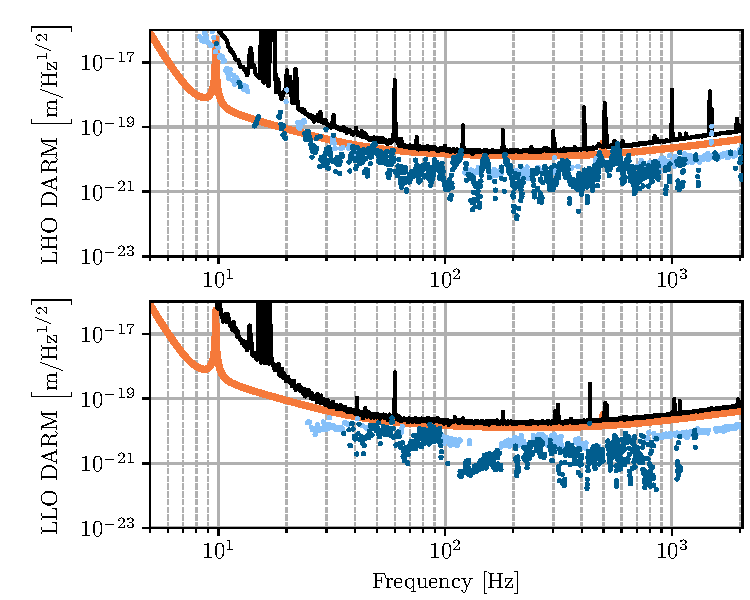
\includegraphics[width=\textwidth]{figures/ambient_vib.pdf}
	\caption{
		Ambient estimate of vibrational noise levels at LHO (top) and LLO (bottom).}
	\label{fig:ambient-vib}
\end{figure}

Figure~\ref{fig:ambient-vib} shows the ambient contribution of vibrational noise during \ac{O3}, produced by combining the highest coupling factors among accelerometers and microphones measured from an injection campaign at the beginning of \ac{O3}.
At the end of \ac{O3}, the vibration noise background at both observatories was dominated by input beam jitter above 100\,Hz (discussed in Section~\ref{sec:jitter}).
At \ac{LHO},  the dominant coupling region below 100\,Hz was the output arm.
At \ac{LLO}, the dominant coupling regions were the Y-end in the 40-60\,Hz band and the output arm in the 60-100\,Hz band.

\subsection{Input beam jitter}

\begin{figure}
	\centering
%	\includegraphics[width=\textwidth]{}
	\caption{Improvement in jitter coupling at LHO (left) and LLO (right) between the start and end of O3.}
	\label{fig:jitter}
\end{figure}

\subsection{Scattered light at the HAM5/6 septum}

\subsection{Search for the source of a 48-Hz peak}

\begin{figure}
	\centering
	\includegraphics[width=\textwidth]{figures/48Hz.png}
	\caption{LHO DARM spectrum before and after mitigation of the 48-Hz peak.}
	\label{fig:48hz}
\end{figure}

\section{Magnetic noise studies during O3}

\begin{figure}[h!]
	\centering
	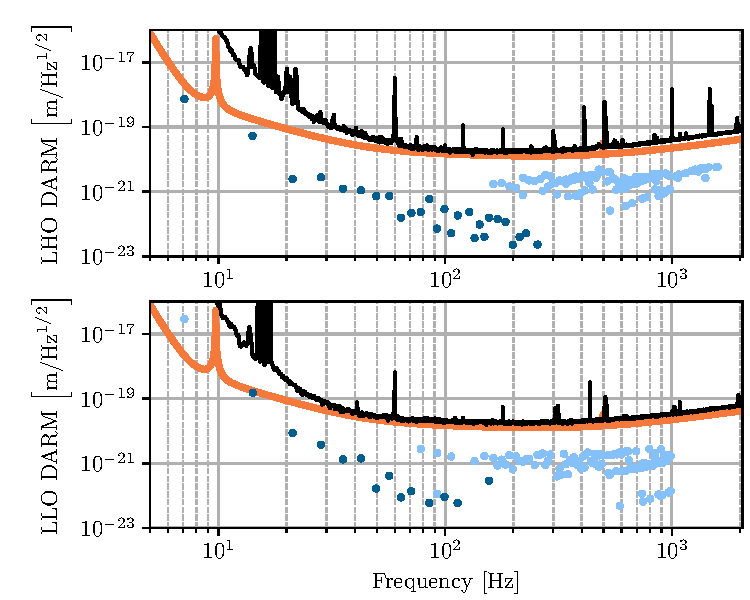
\includegraphics[width=\textwidth]{figures/ambient_mag.pdf}
	\caption{
		Ambient estimate of magnetic noise levels at LHO (top) and LLO (bottom).}
	\label{fig:ambient-mag}
\end{figure}

Magnetic injections early in \ac{aLIGO} suggested that coupling to permanent magnets in the suspension system  could prevent \ac{LIGO} from reaching design sensitivity in the 10-20\,Hz regions~\cite{Schofield_2013}.
While the test mass actuator is electrostatic and not magnetic (as in \ac{iLIGO}), a number of permanent magnets were used in the suspensions, including for actuation in the first three of the four levels of the isolation chain and for eddy current damping.
The greatest number of permanent magnets were in the eddy current damping arrays and these were removed.
Nevertheless, ambient fields are still predicted to produce noise at greater than one-tenth of the design sensitivity in the 10-20\,Hz band (Figure~\ref{fig:ambient-mag}), and may need to be further addressed as we reach design sensitivity in the 10\,Hz region.

At higher frequencies, generally above about 30\,Hz, the dominant magnetic coupling appears to be through induction of currents in cables and at connectors, mainly to actuator cabling and other cabling in the control system.
Mitigation of coupling to cables and connectors has required a continuing program of monitoring coupling since cables are often disconnected and reconnected during runs as electronics are replaced for problems or upgrades.
This program consists of making weekly, broadband magnetic field injections using the large wall-mounted coils described in Section~\ref{sec:magnetic-injections}.
The injections have shown that peaks can appear or disappear, as well as shift in frequency, on a weekly basis.

\subsection{Fluctuations in magnetic coupling}

\begin{figure}
	\centering
%	\includegraphics[width=\textwidth]{}
	\caption{
		Ambient estimate of magnetic noise levels at LHO on Mar \XX, 2019 (blue), \XX weeks before O3, and on Apr \XX, 2019 (orange), \XX weeks into O3.}
	\label{fig:weekly-mag-preO3}
\end{figure}

\begin{figure}
	\centering
%	\includegraphics[width=\textwidth]{}
	\caption{Weekly trends in frequency (top) and amplitude (top) of peaks in the magnetic coupling functions.}
	\label{fig:weekly-mag-variation}
\end{figure}

\section{Validation of gravitational wave event candidates}\label{subsec:vetting}

In addition to investigating sources of environmental influences, knowledge acquired from environmental studies contributes to the vetting of \ac{GW} event candidates.
Analysis pipelines search the strain data for astrophysical signals.
They are categorized into modeled searches for binary mergers that match the data to template waveforms (e.g. GstLAL~\cite{Cannon_2012} and PyCBC~\cite{Usman_2016}) and un-modeled searches that identify excess energy coherent between multiple detectors (e.g. cWB~\cite{Klimenko_2008}, oLIB~\cite{Lynch_2017}, and BW~\cite{Cornish_2015}).

Contamination of the \ac{GW} data can occur through any of the means discussed in previous sections.
Environmental noise has the potential to be correlated between detectors by stemming from a common source, such as through electromagnetic signals from distant sources or glitches in GPS-correlated electronics.
The analysis pipelines estimate the false-alarm probabilities for GW events based on the background rate of randomly coincident events in the detector network.
They generate background events by time-shifting the data stream of one detector relative to another by time steps much longer than the light travel time between detectors and longer than the duration of GW signals~\cite{Was_2009}.
This method does not account for the possibility of transients being correlated between the detectors due to a common environmental source.

Environmental noise is also particularly relevant to un-modeled searches. Unlike template-based methods, these searches make minimal assumptions about the signal waveform and rely more heavily on signal correlation between sites.

The first observation of a \ac{GW} occurred on 14 Sept 2015~\cite{gw150914}.
The event, a short-duration binary black hole merger designated GW150914, required a number of follow-up investigations to find potential noise sources around the time of the event~\cite{Detchar_2016}.
This included an examination of the status of all \ac{PEM} sensors and any significant signals they observed for possible contamination of the GW signal~\cite{Schofield_150914}.
A few of the \ac{PEM} sensors were not working, but because of redundancy, coverage was sufficient. 

Comparisons between Q-transform spectrograms~\cite{Chatterji_2004} of all coincident events in environmental sensors to the time-frequency path of the event revealed that no environmental signals had paths similar to the event candidate.
Q-transforms produce a quality-factor-optimized logarithmic tiling of the time-frequency space, making them useful for visualizing transients.
The \acp{SNR} of the matching signals were also compared to that of the event, showing that even if there were overlapping time-frequency paths, none of the environmental signals were large enough to influence the strain data at the \ac{SNR} level of the event, based on multiplying the environmental signals by their respective sensor coupling functions.

The validation process for novel events such as GW150914 also includes redundant checks for global sources of environmental noise.
We use a dedicated cosmic ray detector located below an input test mass at \ac{LHO} to examine any association of cosmic ray showers to excess noise in \ac{DARM}.
We also check external observatories for coronal mass ejections, solar radio signals, geomagnetic signals, and \ac{RF} signals in the detection band as well as higher frequencies.

There was specific concern over a co-incident extremely-high current (504\,kA) lightning strike over Burkina Faso, prompting additional studies of the effects of lightning on the interferometer~\cite{Schofield_lightning}.
Investigations of similar strikes found no effect on the strain data and investigations of closer strikes confirmed that the magnetometers were much more sensitive to lightning strikes than the interferometer was.
In conclusion there was no reason to veto the first detection based on environmental disturbances.

Subsequent detections throughout \ac{O1} and \ac{O2} employed a similar procedure; however the development of the method described in Section~\ref{sec:cf} for producing coupling functions for all sensors expedited the process.
This was especially important for examining environmental noise during GW170817, the first long-duration event detected by \ac{LIGO}~\cite{gw170817, Schofield_170817}.
The longer duration of this event (75\,s) unsurprisingly overlapped with many environmental signals.
Based on the coupling functions for those sensors, several of these environmental events were loud enough (estimated \ac{DARM} signals of up to SNR~4) to have contributed to the interferometer readout, but not enough to account for the \ac{GW} signal.
Furthermore, none of them had a time-frequency morphology that correlated with any features in the candidate signal.

Since \ac{O3}, most of the procedure described above has been automated in order to handle the increase in detection rate.
The automated vetting is performed by the \code{pemcheck} routine, which is a part of the \ac{DQR}.
When an event is detected by the astrophysical search pipelines, a \ac{DQR} is initiated and assembles a plethora of tasks for assessing the data quality at each observatory during the time of the event.
Among these tasks, an omega scan pipeline~\cite{Davis_2021, Chatterji_2004} is used to search for transient noise in all \ac{PEM} sensors in the time window spanning the event candidate.
It does so by producing a Q-transform for each sensor and reporting those in which there is a transient signal with a false-alarm rate below $10^{-3}$\,Hz.
The omega scan also reports the frequency and amplitude of the most significant tile for each sensor.
The \code{pemcheck} uses the output of the omega scan to estimate each sensor's potential affect on the data quality of the detector.
The coupling function of each sensor is interpolated at the peak frequency and multiplied by the peak amplitude, producing an estimated \ac{DARM} amplitude.

Sensors whose estimated contribution exceed one tenth of the \ac{DARM} background level are flagged for human input, requiring a comparison of the environmental signal morphology to that of the event candidate.
If there is sufficient signal overlap, reviewers may advise that analysts perform some noise removal in the data, such as by gating or filtering out the appropriate time or frequency range, before performing further follow up analyses.
The event could be retracted, if gating or filtering out the environmental contribution would reduce the signal-to-noise ratio of the candidate to a level no longer consistent with a GW detection.

During \ac{O3}, no candidates were retracted on the basis of the environmental coupling check alone.
Some human input was still required for all of the \XX events reported in Abbott et al.\ (2020)~\cite{gwtc2}, although little to no signal overlap of environmental transients was seen.
